%{{{
\documentclass{beamer}
\usetheme{ensam}
\usepackage{pgfplots}
\usepackage{subcaption}
\usepackage{acronym}
\usepackage{tikz}
\usetikzlibrary{calc}
\usepackage{amsmath}
\usepackage {algorithmic}
\usepackage{algorithm}
\usepackage{eqparbox}
\usepackage[font=scriptsize]{caption}
\usetikzlibrary{bayesnet,positioning,calc}
\tikzstyle{obs} = [latent,fill=lightBlue]
\tikzstyle{default}=[draw=sexyRed,thick,rounded corners,text width=0.5in,font=\scriptsize,align=center]
\usepgfplotslibrary{colorbrewer}
\definecolor{ForestGreen}{RGB}{34,139,34}
\newcommand{\comment}[1]{\textcolor{ForestGreen}{#1}}
%algorithmic comment
\renewcommand\algorithmiccomment[1]{%
  \hfill\comment{\#\scriptsize\eqparbox{COMMENT}{#1}}%
}
\renewcommand{\algorithmicrequire}{\textbf{Input:}}
\renewcommand{\algorithmicensure}{\textbf{Output:}}
\title{Variable Aleatoire discrete}
\author{\underline{A.Belcaid}}
\institute{\small ENSA-Safi} 

%tikz bayesian theme
\usetikzlibrary{bayesnet,positioning,calc}
\tikzstyle{obs} = [latent,fill=lightBlue]
\tikzstyle{default}=[draw=sexyRed,thick,rounded corners,text width=0.5in,font=\scriptsize,align=center]
\DeclareMathOperator{\argmin}{argmin}

\pgfplotsset{every tick label/.append style={font=\tiny}}



%acronyms
\acrodef{VA}{Variable Aléatoire}



\begin{document}
\maketitle

\begin{frame}
\tableofcontents
\end{frame}

\section{Variable aléatoire}
\begin{frame}[t]
  \frametitle{Introduction}

  \begin{center}
  \begin{tikzpicture}[scale=1,>=latex]
    \node [blue](A) at (0,0) {a};
    \node [sexyRed](B) at (1,0) {b} ;
    \node[lightBlue] (C) at (2,0) {c};
    \node[sexyRed] (D) at (3,0) {d};
    \draw[thick ] (-.5,-.5) rectangle ( 3.5, 0.6);

    \only<2->{
    \draw[thick, sexyRed,->] (-2,-2) -- (2,-2)node[label=above:$w$]{};
    \draw[thick, blue] (A) to[bend left=30] (-1, -2)node[label=below:{$62$}]{}; 
    \draw[thick, lightBlue] (C) to[bend left=20] (0, -2)node[label=below:{$75$}]{}; 
  }
  \only<3->{
  \node[sexyRed] at (-1,-1) {$\large W$};}
    \only<5->{
    \draw[thick, lightBlue,->] (3,-2) -- (6,-2)node[label=above:$H$]{};
    \draw[thick, blue] (A) to[bend right=10] (3.5, -2)node[label=below:{$1.7$}]{}; 
    \draw[thick, lightBlue] (C) to[bend right=20] (5, -2)node[label=below:{$1.8$}]{}; 
  }
    
  \end{tikzpicture}
  \end{center}
\only<4->{
  {
    On peut penser a $W$ comme une boite noire :
  }
}
\vspace*{1cm}
  \begin{center}
  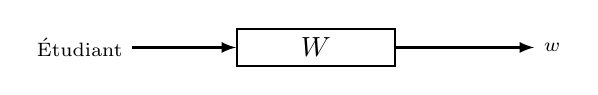
\begin{tikzpicture}[scale=1, transform shape]
    \only<4->{
    \node at ( 0,0) (E) {\scriptsize Étudiant};
    \node[thick, minimum width=2cm,draw] (W) at (3,0){$W$};
    \node at ( 6,0) (w) {\scriptsize $w$};
    \path[thick,draw,->,>=latex](E)--(W);
    \path[thick,draw,->,>=latex](W)--(w);
  }
  \end{tikzpicture}
  \end{center}
 
\end{frame}

\begin{frame}[<+->]
  \frametitle{Formalisme}
  
  \begin{itemize}
    \scriptsize
    \item Une \acf{VA} est une fonction qui associe une valeur a chaque
      \textbf{etat} d'une expérience aléatoire.\\[4pt]
    \item Mathématiquement on l'as représente comme:
      \begin{equation*}
        \begin{array}{llll}
          X & \Omega & \longrightarrow & \mathbb{R}\\[4pt]
        \end{array}
      \end{equation*}

    \item L'espace d'état peut être \alert{\textbf{discret}}  ou
      \textbf{continu}.\\[4pt]
      \pause
     \begin{minipage}{0.6\textwidth}
      \begin{block}{Notation}
        Variable aléatoire \alert{$X$}        \quad\quad valeur numérique \alert{$x$}
     \end{block}
   \end{minipage}
 \item On peut avoir plusieurs \ac{VA}  associés a la même expérience
   aleatoire.\\[4pt]
  \item Une fonction d'une ou plusieurs \ac{VA} est aussi une \textbf{variable
    aléatoire}
   $$ B = \frac{W}{H^2}$$
  \end{itemize}
\end{frame}


\section{Loi de probabilité}

\begin{frame}[t]
  \frametitle{Loi de probabilité}
\begin{columns}
  \begin{column}{0.6\textwidth}
   \begin{itemize}
     \scriptsize
     \item<1-> C'est la loi de distribution de chaque valeur de $X$.\\[4pt]
     \item<2-> Pour une variable discrète on la représente sous forme d'
       \alert{\textbf{histograme}}.\\[4pt]
       \vspace*{.3cm}
       \only<3->{
 
         \begin{block}{Définition}
          $$
          p_X(x) = \mathbf{P}(X=x) = \mathbf{P}\left(\left\{ w \in \Omega\; |\;
          X(w) = x \right\}\right)
           $$
         \end{block}
         }
      \only<4->
      {
        \begin{center}
        \begin{tikzpicture}[scale=.7]
          
          \path[draw, thick, ->, >= latex] (0,0) -- (5,0)node[label=below:$x$]{};
          \path[draw, thick, ->, >= latex] (0,0) -- (0,4)node[label=left:$P_X$]{};
          \node [minimum width=3pt, inner sep=0,
            label=below:3,draw,circle,fill=gray] (x3) at (2,0) {};
          \node [minimum width=3pt, inner sep=0,
            label=below:4,draw,circle,fill=gray] (x4) at (3,0) {};
          \node [minimum width=3pt, inner sep=0,
            label=below:5,draw,circle,fill=gray] (x5) at (4,0) {};

          \path[draw,sexyRed, very thick] (x3) -- (2,1)node[label=above:$\frac{1}{4}$]{};
          \path[draw,sexyRed, very thick] (x4) --
            (3,1)node[label=above:$\frac{1}{4}$]{};
          \path[draw,sexyRed, very thick] (x5) --
            (4,2)node[label=above:$\frac{1}{2}$]{};

          \node at (1.5,3) {\scriptsize $\displaystyle\sum_x p_X(x) =  1$};
        \end{tikzpicture}
        \end{center}
      }

   \end{itemize} 
  \end{column}
  \begin{column}{0.4\textwidth}
  \begin{center}
  \begin{tikzpicture}[scale=.7]
  \draw[thick, fill=yellow!40] (0,0) rectangle (2,-3);
  \node[draw, label=left:a, fill=gray, minimum width=4pt,circle, inner sep=0pt]
    (A) at (1,-.5) {};
  \node[draw, label=left:b, fill=gray, minimum width=4pt,circle, inner sep=0pt]
    (B)  at (1.5,-1.2) {};
  
  \node[draw, label=right:c, fill=gray, minimum width=4pt,circle, inner sep=0pt]
    (C)  at (.2,-1.9) {};
  \node[draw, label=left:d, fill=gray, minimum width=4pt,circle, inner sep=0pt]
    (D)  at (1.5,-2.5) {};
  \node[sexyRed] at (.7, 0.4) {$\Omega$};
  \only<2->
  {
    \path[draw, thick, >= latex,->] (4,-4) -- (4,1);
  \node[draw, label=right:5, fill=gray, minimum width=2pt,circle, inner sep=0pt]
    (x5) at (4,-.7) {};

  \node[draw, label=right:4, fill=gray, minimum width=2pt,circle, inner sep=0pt]
    (x4) at (4,-2) {};

  \node[draw, label=right:3, fill=gray, minimum width=2pt,circle, inner sep=0pt]
    (x3) at (4,-3) {};
  \path[thick, ->, > = latex, draw, sexyRed] (A) -- (x5);
  \path[thick, ->, > = latex, draw, sexyRed] (B) -- (x5);
  \path[thick, ->, > = latex, draw, sexyRed] (C) -- (x4);
  \path[thick, ->, > = latex, draw, sexyRed] (D) -- (x3);
  \node at (4, 1.5) {$X$};
}
  
\end{tikzpicture}
\end{center}
\end{column}
\end{columns}
\end{frame}


\begin{frame}[t]
  \frametitle{Exemple de calcul}
\begin{itemize}
  \item On considère notre exemple classique de lance d'un dé a
    \alert{\textbf{quatre faces}}.
   \begin{center}
   
\begin{tikzpicture}[scale=1, transform shape]
     
     \draw[thick](0,0) grid (4,4);
   \end{tikzpicture}
   \end{center}

   \begin{enumerate}
     \scriptsize
     \item On considère la variable aléatoire 
       $$
       Z = X + Y
       $$
     \item  Calculer la probabilité $P_Z(3)$.\\[4pt]
     \item Compléter tout l'histogramme de cette variable.
   \end{enumerate}
    
\end{itemize}
  
\end{frame}
\subsection{Bernoulli}
\begin{frame}[t]
  \frametitle{Bernoulli}
  \begin{itemize}
    \scriptsize
    \item L'exemple le plus simple d'une variable discrète avec un
      \alert{\textbf{parametre $p\in [0,1]$}} 
      \pause
      \vspace*{.5cm}
      \begin{columns}
        \begin{column}{0.5\textwidth}
         \begin{equation*}
           X = \left\{
             \begin{array}{l l}
               1  & \text{\tiny avec probabilite } p\\[4pt]
               0  & \text{\tiny avec probabilite } 1-p
             \end{array}
           \right.
         \end{equation*} 
        \end{column}
        \begin{column}{0.5\textwidth}
          \begin{center}
          \begin{tikzpicture}[scale=1, transform shape]
            
            \path[draw, ->, > = latex,thick](-0.5,-.5) -- (3,-.5);
            \path[draw, ->, > = latex,thick](-.5,-.5) -- (-0.5,1);
            \path[draw, ->, > = latex,thick,sexyRed,](0,-.5) --
              (0,.7);

            \path[draw, ->, > = latex,thick,sexyRed,](1,-.5) --
              (1,.3);
            \node at (0,-.7) {0};
            \node at (0,.8) {\tiny$1-p$};
            \node at (1,-.7) {1};
            \node at (1,.4) {\tiny$p$};
          \end{tikzpicture}
          \end{center}
        \end{column}
      \end{columns}
        \item Cette variable modélise une expérience aléatoire de
          (succès/échec).\\[4pt]

        \item Aussi très utile comme fonction indicatrice d'un
          \textbf{évènement}
        
          \begin{equation*}
            I_A = 1 \iff \text{A est realise}
          \end{equation*}
          \pause
          \begin{columns}
            \begin{column}{0.5\textwidth}
              \begin{center}
              \begin{tikzpicture}[scale=1, transform shape]
                \draw[sexyRed, thick] (0,0) rectangle (3,2) ;
                \draw[thick, sexyRed] (0,1) .. controls (1.5,2) and (2.3,-.4)
                  .. (3,1);
                \node at (1.5, 0.5) {$A^c$};
                \node at (1.5, 1.5) {$A$};
                \path[draw, thick, > = latex, ->] (4,0)  -- (4, 2.5);
                \node[minimum width=4pt, inner sep=0pt, fill,circle,
                  label=right:0]  (0) at (4,1){};
                \node[minimum width=4pt, inner sep=0pt, fill,circle,
                  label=right:1]  (1) at (4,2){};
                \node [minimum width=4pt, inner sep=0pt,fill, circle] (p1) at
                  (2.5, 1.5) {};
                \node [minimum width=4pt, inner sep=0pt,fill, circle] (p2) at
                  (1.7, 1.3) {};
                \node [minimum width=4pt, inner sep=0pt,fill, circle] (p3) at
                  (0.7, 0.3) {};

                \node [minimum width=4pt, inner sep=0pt,fill, circle] (p4) at
                  (2.7, 0.3) {};
                \edge[lightBlue,-,dotted]{1}{p1,p2}
                \edge[black,-,dotted]{0}{p3,p4}
              \end{tikzpicture}
              \end{center}
            \end{column}
            \begin{column}{0.5\textwidth}
             $$
             \mathbf{P}_{I_A} = \mathbf{P}(I_A = 1) = \mathbf{P}(A)
             $$

            \end{column}
          \end{columns}
  \end{itemize}
  
\end{frame}
\subsection{Uniforme}

\begin{frame}[<+->]
  \frametitle{Loi discrète uniforme}
  
  \begin{itemize}
    \scriptsize
    \item \textbf{Paramètres} : entiers \alert{\textbf{a, b}}; $a \le b$.\\[12pt]
    \item \textbf{Expérience} : Tirer un élément de $\{a, a+1, \ldots, b\}$. Tous
      équiprobable.\\[12pt]
    \item \textbf{Espace d'états}: $\{a, a+1, \ldots, b\}$.\\[12pt]
    \item \textbf{Variable aleatoire}: $X:\;\; X(w) = w$
    \item \textbf{Modele de} : ignorance complète!!
  \end{itemize}
  \vspace*{.5cm}
  \begin{columns}
    \begin{column}{0.5\textwidth}
      \begin{center}
      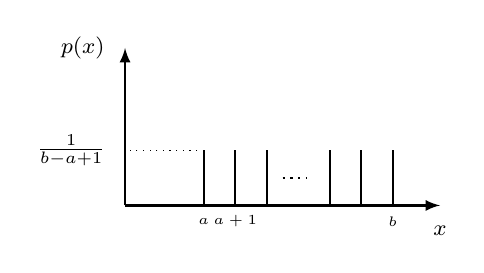
\begin{tikzpicture}[scale=1,>= latex]
        
        \path[draw,thick, ->] (0,0) -- (4,0)node[label=below:$\tiny x$]{};
        \path[draw,thick, ->] (0,0) -- (0,2)node[label=left:$\tiny p(x)$]{};
        \path[draw,thick] (1,0) -- (1,.7);
        \path[draw,thick] (1.4,0) -- (1.4,.7);
        \path[draw,thick] (1.8,0) -- (1.8,.7);
        \node at (1,-.2){\tiny$a$};
        \node at (1.4,-.2){\tiny$a+1$};
        \path[dotted,draw,thick] (2,0.35) -- (2.3,.35);
        \path[draw,thick] (3,0) -- (3,.7);
        \path[draw,thick] (2.6,0) -- (2.6,.7);
        \path[draw,thick] (3.4,0) -- (3.4,.7);
        \node at (3.4,-.2){\tiny$b$};
        \path[draw,thick] (1.8,0) -- (1.8,.7);
        \path[dotted,draw] (1,.7) -- (0,.7)node[label=left:{$\frac{1}{b-a+1}$}]{};
      \end{tikzpicture}
      \end{center}
    \end{column}
    \begin{column}{0.5\textwidth}
\begin{center}
  \scriptsize
  \textbf{Cas spécial} $a = b$.
\begin{tikzpicture}[scale=.8, > = latex]
  
        \path[draw,thick, ->] (0,0) -- (4,0)node[label=below:$\tiny x$]{};
        \path[draw,thick, ->] (0,0) -- (0,2)node[label=left:$\tiny p(x)$]{};
        \path[draw,thick] (2,0) -- (2,1);
        \node at (2,-.2){a};
        \path[dotted,draw] (2,1) -- (0,1)node[label=left:{$1$}]{};
\end{tikzpicture}
\end{center}
    \end{column}
  \end{columns}
\end{frame}
  
\subsection{Binomiale}
\begin{frame}[t]
  \frametitle{Variable Binomiale}
  \textbf{\structure{Variable Aléatoire Binomiale}}  
  \begin{itemize}
    \scriptsize
    \item \textbf{Experience}: $n$ répétition d'expériences Bernoulli identiques  et
      \alert{\textbf{independents}}.\\[8pt]
    \item \textbf{Parametres}: \alert{\textbf{n}}: nombre de répétition, $p$
      probabilité de succès.\\[8pt]
    \item \textbf{Espace D'états}: Ensemble de (S\{succès\}, E\{Échecs\}) de
      longueur $n$. \\[8pt]
    \item \textbf{Variable aléatoire} $X$ : Nombre de succès.\\[8pt]
    \item \textbf{Modélise}: Nombre de cas \alert{réussi} dans une répétition
      identique et \alert{\textbf{indépendants}}.\\[8pt]
  \end{itemize}
  \vspace*{0.2cm}
  \begin{columns}
    \begin{column}{0.5\textwidth}
      
        \centering
        \includegraphics[width=0.8\textwidth]{./binomial.png}
    \end{column}
    \begin{column}{0.5\textwidth}
      \pause
       \small
     \begin{equation*}
       p_X(k) = \binom{n}{k}p^k(1-p)^{n-k}
     \end{equation*} 
    \end{column}
  \end{columns}
\end{frame}

\begin{frame}[t]
  \frametitle{Exemples Binomiale}
    \begin{figure}
    \centering
    \includegraphics[width=0.9\textwidth, height=6cm]{./binomial_set.png}
    \caption{Illustration des distributions Binomiale pour différentes paramètres
    $(n,p)$}
    \label{fig:binom}
  \end{figure}
\end{frame}
\subsection{Geometrique}

\begin{frame}[t]
  \frametitle{Loi Geometrique}
  \textbf{\structure{Loi géométrique}}
  \begin{itemize}
    \scriptsize
    \item \textbf{Expérience}: Répétition \alert{\textbf{infinie}} d'une
      Bernoulli.\\[8pt]
    \item \textbf{Paramètres} $\alert{p}$ paramètre succès de Bernoulli.
    \item \textbf{Espace d'états}: Une suite infinie de
      \{S(succès),E(Échec)\}\\[8pt]
    \item \textbf{Modelise} : Temps d'attente jusqu'à un
      \alert{\textbf{succès}}\\[12pt]

    \pause
    \begin{columns}
      \begin{column}{0.5\textwidth}
      \begin{itemize}
        \item $\mathbf{P}_X(k) =$ \\[2cm]
        \item $\mathbf{P}(\text{pas de succès})$ 
      \end{itemize}
      \end{column}
      \begin{column}{0.5\textwidth}
          \centering
          \includegraphics[width=0.8\textwidth]{./geometric.png}
      \end{column}
    \end{columns}
  \end{itemize}
\end{frame}
\section{Esperance}

\begin{frame}[t]
  \frametitle{Espérance d'une variable aléatoire}

  \begin{columns}
    \begin{column}{0.5\textwidth}
      \begin{itemize}
        \scriptsize
        \item<1-> \textbf{Motivation}: On joue a un jeu $1000$ fois. Le gain
          aléatoire est décrit comme:
        \item<3-> Quel sera la gain \alert{\textbf{moyen}}?\\[2cm]
        \item<4-> 
          \begin{block}{Définition}
            $$
            E[X] = \sum_x x p_x(x)
            $$
          \end{block}
      \end{itemize}
    \end{column}
    \begin{column}{0.5\textwidth}
      
    \only<2->{
      \begin{equation*}
        \scriptsize
      X = \begin{cases}
        1 & \text{a.p } \frac{2}{10} \\[6pt]
        2 & \text{a.p } \frac{5}{10} \\[6pt]
        4 & \text{a.p } \frac{3}{10} \\[6pt] 
      \end{cases}
      \end{equation*}
    }
    \only<5->
    {
      \begin{itemize}
        \scriptsize
        \item \textbf{Interprétations}: Moyen d'un grand nombre de répétition
          \alert{\textbf{indépendant}}  répétition.
      \end{itemize}
    }
    \end{column}
  \end{columns}

  \pause
  \begin{itemize}
    \scriptsize
    \item \alert{\textbf{Attention}}: Si on dispose d'une somme
      \textbf{infinie}, alors il faut qu'elle soit bien définie:

      $$
      \sum_x \vert x\vert p_X(x) < \infty
      $$
  \end{itemize}
\end{frame}

\begin{frame}[t]
  \frametitle{Espérance d'une Bernoulli}
      \small
      \begin{itemize}
        \item
      \begin{equation*}
       X = \begin{cases}
         1 & \text{a.p  } p\\[6pt]  
         0 & \text{a.p  } 1 - p
       \end{cases}
      \end{equation*}
      \vspace*{.5cm}
      \pause
       \begin{equation*}
         E[X] = 1\cdot p + 0\cdot (1-p) = p
       \end{equation*}
       \pause
     \item Si $X$ est l'indicatrice de $A$, \alert{\textbf{$X = I_A$}}.\\[.5cm]
        \pause
        $X$ est un Bernoulli avec $p = \mathbf{P}(A)$
        \begin{equation*}
          E[I_A] = \mathbf{P}(A)
        \end{equation*}
   \end{itemize}
\end{frame}

\begin{frame}[t]
  \frametitle{Espérance d'une variable uniforme}
  
  \begin{itemize}
    \item Une loi uniforme de $0,1,\ldots, n$.\\[12pt]
  \end{itemize}
  \pause
    \centering
    \small
    \includegraphics[width=0.5\textwidth]{./uniform_0_n.png}
    \pause
    \begin{eqnarray*}
      E[X] & = & \sum_{x=0}^n x p_X(x)\\
           & = & \frac{1}{n+1}\cdot (0 + 1 + 2 + \ldots + n)\\
           & = & \frac{1}{n+1}\frac{n(n+1)}{2}\\
           & = & \frac{n}{2}
    \end{eqnarray*}
\end{frame}


\begin{frame}[<+->]
  \frametitle{Espérance comme moyenne}
  
  \begin{itemize}
    \scriptize
    \item \alert{\textbf{$n$}} étudiants.\\[6pt]
    \item Note de chaque étudiant \alert{\textbf{$x_i$}}.\\[6pt]
    \item On suppose que les notes sont distribues uniformément:\\[6pt]
      \begin{itemize}
        \item \alert{\textbf{\mathbf{P}_X(x_i)}}:\\[12pt]
        \item \alert{\textbf{$E[X]$}}:
      \end{itemize}
  \end{itemize}
\end{frame}

\begin{frame}[<+->]
  \frametitle{Propriété}
 \begin{itemize}
   \item Si \alert{\textbf{$X \geq 0$}} alors 
     $$
     \mathbf{E}[X] \geq 0
     $$
     \vspace*{1cm}
   \item Si \alert{\textbf{$a \leq X \leq b$}}  alors:

     $$
     a \leq \mathbf{E}[X] \leq b
     $$
     \vspace*{1cm}
   \item Si $c$ est une constante, alors
     \begin{equation*}
       \mathbf{E}(c) = c
     \end{equation*}
 \end{itemize} 
\end{frame}



\begin{frame}[t]
  \frametitle{Espérance d'une fonction de VA}

  \begin{columns}
    \begin{column}{0.5\textwidth}
      \begin{itemize}
        \scriptsize
        \item<1-> Soit \alert{\textbf{X}}  et \alert{$Y = g(X)$}.\\[12pt]
        \item<2->  Moyenne en utilisant $y$.
          $$
          \mathbf{E}[Y] = \sum_y y P_Y(y)
          $$
        \item<3-> Moyenne en utilisant $x$.
          \begin{equation*}
            E[Y] = E[g(X)] = \sum_x g(x) \mathbf{P}_X(x)
          \end{equation*}
        \item<4->
          \begin{eqnarray*}
            \mathbf{E}[Y] &=& \sum_y \sum_{x: g(x)=y}g(x)P_X(x) \\
                          &=& \sum_y \alert{y}\sum_{x: g(x)=y}P_X(x)\\
                          &=& \sum_y y P_Y(y)
          \end{eqnarray*}
      \end{itemize}
    \end{column}
    \begin{column}{0.5\textwidth}
       \centering
       \only<2->{
       \includegraphics[width=0.8\textwidth]{./esperance_g.png}
     }
     \only<5->{
     \begin{itemize}
       \scriptsize
       \item $\mathbf{E}[X^2]$ = \\[12pt]
        \item \alert{Attention} En général
          $$
          \mathbf{E}[g(X)] \neq g(\mathbf{E}[X])
          $$
     \end{itemize}
   }
    \end{column}
  \end{columns}
\end{frame}

\begin{frame}[t]
  \frametitle{Linéarité d'espérance}
 \begin{block}{Linéarité d'espérance}
  \begin{equation*}
  \mathbf{E}[aX + b] = a\mathbf{E}[X] + b
  \end{equation*} 
 \end{block} 
 \begin{itemize}
   \item Intuitive.\\[4pt]
   \item Démontrer ce résultat.
 \end{itemize}
\end{frame}
\end{document}
